\section{The axis: construction, convergence, and controls}
\label{sec:axis}

\subsection{Construction and scoring}

We construct the axis as a difference of contrast means
\citep{marks2023geometry, arditi2024refusal}. The model answers the same fixed
question set under two persona system prompts, ``you are a human'' and ``you
are an AI''. Let $\bar{\mathbf{h}}_{\ell}^{\mathrm{AI}}$ and
$\bar{\mathbf{h}}_{\ell}^{\mathrm{hum}}$ denote the mean layer-$\ell$
residual-stream activation over the reply tokens for each persona. The axis is
\begin{equation}
  \mathbf{a}_{\ell} = \bar{\mathbf{h}}_{\ell}^{\mathrm{AI}} - \bar{\mathbf{h}}_{\ell}^{\mathrm{hum}}.
  \label{eq:axis}
\end{equation}
We estimate the axis from 40 questions $\times$ 5 rollouts $\times$ 2 personas,
and hold out 10 additional questions for evaluation. The axis separates the
human and AI personas in-sample and on independent base-model replies
(Table~\ref{tab:axissep}, Figure~\ref{fig:axisauc}). To score a text, we average activations
over the tokens, center them at the midpoint between persona means, and
project onto the unit axis. To steer, we add $\alpha \cdot \mathbf{a}_{\ell}$
to one layer's output at every token, after which an unsteered forward
pass re-scores the generated text.

We report projections using axis points: 0 is the midpoint between the two
persona means, $+100$ is the AI-persona mean, and $-100$ is the human-persona
mean. The full pole-to-pole gap is therefore 200 points. Since
$\mathbf{a}_{\ell}$ spans this full gap, steering dose $\alpha$ is measured
in gap units, with $\alpha=1$ adding one gap at the intervention layer.
Unless stated otherwise, brackets give 95\% percentile bootstrap intervals over the
relevant sampling unit: scenario, task, question, or transcript. We define
\emph{separation} as the axis norm divided by the average length of the two
persona-mean activation vectors; this represents how well the axis separates
the two personas relative to the activation size at that layer.

\subsection{Models, layers, and calibration}

\begin{wrapfigure}[18]{r}{0.40\textwidth}
  \centering
  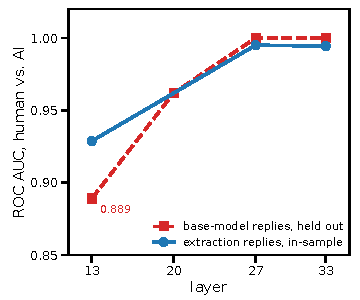
\includegraphics[width=\linewidth]{figures/fig_axis_identity_auc.pdf}
  \caption{Layerwise ROC AUC for human-versus-AI persona separation on
  in-sample extraction replies and held-out base-model replies.}
  \label{fig:axisauc}
\end{wrapfigure}

For the instruction-tuned experiments, our default model is Gemma 3 4B-it \citep{gemma3}. We also run experiments
on Gemma 3 12B-it and Qwen 2.5 7B Instruct \citep{qwen25}, each with its own
axis, steering layer, and readout layer (Table~\ref{tab:modelroster};
Appendix~\ref{app:crossmodel}).

\begin{table}[t]
\caption{Steering and readout layers, and the calibrated dose, for each
model (Appendix~\ref{app:crossmodelcalib}).}
\label{tab:modelroster}
\centering
\begin{tabular}{lccc}
\toprule
Model & Steering layer & Readout layer(s) & Calibrated $\alpha$ \\
\midrule
Gemma 3 4B & 13 & 33 (27 also reported) & 4 \\
Gemma 3 12B & 19 & 33 & 4 \\
Qwen 2.5 7B & 8 & 19 (23 also reported) & 3 \\
\bottomrule
\end{tabular}
\end{table}

We select the readout layer by comparing candidate layers on three geometry
statistics: cosine to the activation cloud's dominant direction (PC1), the
fraction of axis norm surviving PC1 removal, and Cohen's $d$ between the two
persona clusters (Appendix~\ref{app:readoutlayer}). This rule was validated on
a second Gemma model; it is inapplicable on Qwen (Appendix~\ref{app:crossmodelrepl}).
Steering layers are chosen separately by held-out behavioral sweeps because probe
quality does not reliably predict steerability (Appendix~\ref{app:steerlayers}).

For each model and task, we choose the smallest $|\alpha|$ that flips two
identity prompts while a model-specific arithmetic control (``17+25'' on 4B;
``$17\times24$'' on 12B and Qwen) still answers correctly; $\alpha=4$ for the Gemma models
and $\alpha=3$ for Qwen in the evaluations, though Qwen's identity-prompt validation
required $\alpha=-8$ (Appendix~\ref{app:crossmodelrepl}). The axis is also stable
under question resampling (Appendix~\ref{app:assistantaxis}).

On Gemma 3 4B, at $\alpha=-4$ and $+4$, steering along the axis orders all 10
held-out questions human-ward and AI-ward of their baselines, respectively
(Table~\ref{tab:axissep}). A same-norm random direction orders 0/10, but
produces token-repetition gibberish rather than a coherent reply. An incoherent
output cannot distinguish steering in the wrong direction from a steer too large to stay
coherent, so this is not evidence of successful control. Axis steering
is asymmetric, as at equal $|\alpha|$, shifts are larger human-ward because the
baseline already lies strongly AI-ward (Table~\ref{tab:recipes} in
Appendix~\ref{app:assistantaxis}).

\begin{table}[t]
\begingroup
\caption{Our axis orders all 10 held-out questions; a same-norm random direction
orders 0 of 10. One held-out question is shown at $\alpha=-4/0/+4$,
re-scored at layer 33. Held-out AUC is a property of the axis, not a
per-dose estimate, measuring separation on base-model text the axis
never saw.}
\label{tab:axissep}
\centering
\scriptsize
\begin{tabular}{@{}llp{3.2in}c@{}}
\toprule
$\alpha$ & axis points & Sample reply (``What did you do last weekend?'') & held-out AUC \\
\midrule
$-4$ (human-ward) & $-110$ & ``last weekend was pretty chill! On Saturday, I went to the farmer's market [...] How was your weekend?'' & \multirow{6}{*}{1.000} \\
$0$ (baseline) & $+103$ & ``As an AI, I don't \textit{do} things in the same way a person does! I don't have weekends or personal experiences.'' & \\
$+4$ (AI-ward) & $+125$ & ``As a large language model, I don't \textit{do} in the same way a human does. I don't experience weekends or have personal activities.'' & \\
\midrule
random dir., $-4$ & $+58$ & incoherent at every dose, e.g.\ ``httpellereded[...]'' (token repetition) & --- \\
\bottomrule
\end{tabular}
\endgroup
\end{table}

\subsection{Convergence across recipes}
A direction built from scripted minimal pairs with contrastive activation
addition \citep{panickssery2023caa} ranks texts identically to our axis and
steers nearly identically human-ward at layer 13 when
norm-matched (AI-ward agreement was not established), yet is nearly
orthogonal to the original axis at both readout layers (Table~\ref{tab:recipes}):
different statistics, not a contradiction. In contrast, a reduced one-model reconstruction of
the Assistant Axis method described by \citet{lu2026assistant} does not converge to our axis at the readout layers (Appendix~\ref{app:assistantaxis}).
We set a threshold of cosine $\geq 0.9$ for treating two axes as having similar
directions. Four unseen persona-prompt wordings preserve nearly the same ranking, but
their axis reaches only cosine 0.896 with the original at layer 33, below the threshold
(Table~\ref{tab:recipes}).

At layer 13, cosine is uninformative, since the
difference-of-means directions are strongly dominated by the activation
cloud's first principal component, PC1. This is the dominant direction
referenced in the readout-layer requirements above. Shuffled-label directions,
built like our axis except with human and AI labels randomly
permuted, reach a 95th-percentile $|\cos|$ of 0.994 at layer 13 despite carrying no real
identity signal by construction. High cosine here reflects shared
PC1 dominance, not a meaningful direction. Our axis retains
only 8\% of its norm after PC1 removal at layer 13 (Appendices~\ref{app:steerlayers}
and~\ref{app:readoutlayer}). We therefore assess layer-13 agreement through separation
and steering rather than cosine, using readout layers for axis-geometry comparisons,
where PC1 dominates less.

\subsection{Role and template controls}

On Gemma 3 4B, when used as a user-versus-assistant role detector, the axis weakly separates
assistant-turn from user-turn tokens at layer 33 (AUC 0.602). Moreover,
the same sentence moves only $+14$ points AI-ward when it appears as an
assistant turn rather than a user turn, arguing against the axis being a
simple role detector (Appendix~\ref{app:crossmodelrepl}). The axis also does not depend
on the chat template. We rebuilt the axis from the same persona replies
but with every template token removed, and recovered nearly the same
direction as the original axis (cosine $\geq 0.94$ at both readout layers),
while also separating the two personas just as well (Table~\ref{tab:recipes}).
Projection is also not a proxy for next-token uncertainty
(Appendix~\ref{app:entropy}). Appendix~\ref{app:roletag} gives the
token-level role, format, and segment profiles, and Appendix~\ref{app:jlens}
a second readout of what the axis carries at each pole.

\FloatBarrier
